\documentclass[norsk,11pt,a4paper]{article}
\usepackage[T1]{fontenc} % --------------| More characters.
\usepackage[utf8]{inputenc} % ---------| Direct use of scandinavian letters.
\usepackage{float} % --------------------| More options for floats.
\usepackage{graphicx} % -----------------| Support more image formats.
\usepackage{booktabs} % -----------------| Better-looking tables.
\usepackage{tabularx} % -----------------| Better tables
\usepackage{subfig} % -------------------| Subfigures.
\usepackage[a4paper]{geometry} % --------| Adjusting page margins.
\usepackage{amsmath,amssymb,amsfonts} % -| Various math, including eqref.
\usepackage{color} % --------------------| Allows defn. of custom colors.
\usepackage{babel}

% XY-pic. Used for creating illustrations.
\input xy
\xyoption{all}

% Styling captions.
\usepackage{caption}
\captionsetup{margin=10pt,font=small,labelfont=bf}

% Changing section header and title fonts.
\usepackage{sectsty}
\allsectionsfont{\normalfont\sffamily}


%******************************************************************************
% Includes the listings package and sets some settings for it.
% REQUIRES the `color' package.
%******************************************************************************

\usepackage{listings} % -----------------------| Used for source code listings.
\definecolor{lst-gray}{RGB}{100,100,100}  % ---|Color for line-numbers.
\definecolor{lst-light-gray}{RGB}{250,250,250} % Background color for listings.
\definecolor{lst-dark-green}{RGB}{45,111,0} % -| Dark green for comments.
\lstset{
  aboveskip=0em, % -------------------| Skip above listing box.
  backgroundcolor=\color{lst-light-gray}, % Background color.
  basicstyle=\ttfamily\scriptsize, % -| Default font style.
  belowskip=\topskip, % --------------| Skip below listing box.
  breakatwhitespace=false, % ---------| Automatic breaks only at whitespace?.
  breaklines=true, % -----------------| Sets automatic line breaking.
  captionpos=t, % --------------------| Sets the caption-position to bottom.
  commentstyle=\color{lst-dark-green}, % ------| Comment style.
  escapeinside={\%*}{*)}, % ----------| For adding LaTeX within code.
  frame=single, % --------------------| Adds a frame around the code.
  keepspaces=true, % -----------------| Keeps spaces in text.
  keywordstyle=\color{blue}, %--------| Keyword style.
  language={C}, % --------------------| The language of the code.
  literate={æ}{{\ae}}1 % -------------| Character conversions
           {Æ}{{\AE}}1
           {ø}{{\oe}}1
           {Ø}{{\OE}}1
           {å}{{\aa}}1
           {Å}{{\AA}}1
           {µ}{{\ensuremath{\mu}}}1,
  numbers=left, % --------------------| Line-number position: none/left/right.
  numbersep=5pt, % -------------------| Distance between line-numbers and code.
  numberstyle=\tiny\color{lst-gray}, %| The style that used for line-numbers.
  rulecolor=\color{black}, % ---------| Frame color.
  showspaces=false, % ----------------| Show spaces with underscores.
  showstringspaces=false, % ----------| Underline spaces within strings.
  showtabs=false, % ------------------| Show tabs with underscores.
  stepnumber=1, %---------------------| Step between two line-numbers..
  stringstyle=\color{red}, % ---------| String literal style.
  tabsize=4, % -----------------------| Sets default tabsize to 2 spaces.
  title=\lstname % -------------------| Show the filename of included file.
}
%******************************************************************************
% This preabmle contains packages needed to create figures and plots in LaTeX.
%******************************************************************************

\usepackage{etex}
\usepackage{tikz,pgfplots}
\pgfplotsset{compat=1.9}
\usetikzlibrary{arrows,decorations.markings}
\usetikzlibrary{calc}

% Vector Styles for drawings
\tikzstyle{load}   = [ultra thick,-latex]
\tikzstyle{stress} = [-latex]
\tikzstyle{dim}    = [latex-latex]
\tikzstyle{axis}   = [-latex,black!55]


% Figure related stuff
\usepackage{etex}
\usepackage{tikz,pgfplots}
\pgfplotsset{compat=1.9}
\usetikzlibrary{arrows,decorations.markings}


\author{Einar Baumann}
\title{
    \vspace{-1in}
    \usefont{OT1}{bch}{b}{n}
    \normalfont \normalsize \textsc{TKT4140 Numeriske beregninger med datalab} \\ [20pt]
    \vspace{0.1in}
    \rule{\textwidth}{0.5pt} \\[1cm]
    {\sffamily \huge Numerisk løsing av randverdiproblemer med skyteteknikk} \\
    \vspace{0.1in}
    \rule{\textwidth}{2pt} \\[0.7cm]
}

\begin{document}
\maketitle
\thispagestyle{empty}
\clearpage

\section{Lineære ligninger} % (fold)
\label{sec:line_re_ligninger}
Skyteteknikk er en metode til å transformere et randverdiproblem for en ODL til et ekvivalent initialverdiproblem\cite{komp}. Metodens navn stammer fra problemstillingen skissert i Figur~\ref{fig:skyting}.

Mer spesifikt så fungerer metoden ved at man ser på rabndbetingelsene som en funksjon av initialbetingelser i et punkt -- dette reduserer randverdiproblemet til å finne initialbetingelsene som gir en rot.

I Figur~\ref{fig:skyting} vil vi finne vinkelen $\alpha$ som gir skytelengden $x=L$. Vi kjenner her betingelsene for $x=0$ og $x=L$, og det er innlysende at problemet kan løses ved å variere $\alpha$.

\begin{figure}[htbp]
  \centering
  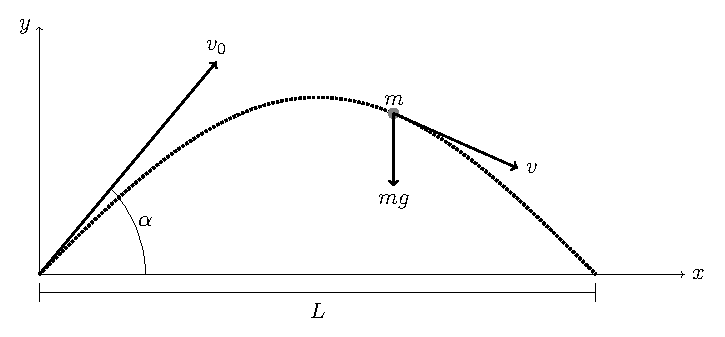
\includegraphics[]{illustrations/shooting.pdf}
  \caption{Illustrasjon av skyting.}
  \label{fig:skyting}
\end{figure}



\subsection{Bestemmelse av randverdi vha. interpolasjon} % (fold)
\label{sub:bestemme_}
Vi ser på et vilkårlig randverdiproblem med randverdier
\begin{equation}
  y(a) = \alpha, \; y(b) = \beta
\end{equation}
Vi velger her å bruke $y(a)=\alpha$ videre som initialbetingelse; i tillegg trenger vi en initialbetingelse for $y'(a)\equiv g(a)$. Ettersom den ikke er kjent må vi ``tippe'' verdier for $y'(a)$ slik at randbetingelsen $y(b)=\beta$ oppfylles. For en 2. ordens \emph{lineær} differensialligning, som de vi ser på i dette kapittelet, er det tilstrekkelig å beregne to verdier for $s=g(a)=y'(a)$. Den rette verdien bestemmer vi deretter ved lineær interpolering.

Setter
\begin{equation}
  \phi(s) = y(b;s) - \beta \label{eq:phi}
\end{equation}
der $s=g(\alpha)$. Den rette verdien $s=s^*$ er funnet når $\phi(s^*)=0$.

Vi begynner med å tippe to verdier $s^{(0)}$ og $s^{(1)}$ og beregner de tilhørende verdiene $\phi^{(0)}$ og $\phi^{(1)}$ med formel \eqref{eq:phi}. Den korrekte verdien $s=s^*$ finnes ved lineær interpolasjon, som vist i Figur~\ref{fig:interpolasjon}.

\begin{figure}[htbp]
  \centering
  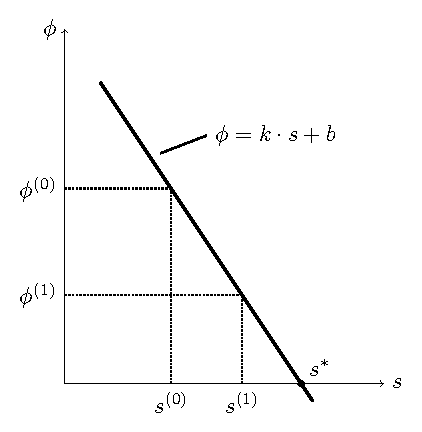
\includegraphics[]{illustrations/interpolation.pdf}
  \caption{En illustrasjon av bruk interpolasjon for bestemmelse av $s^*$.}
  \label{fig:interpolasjon}
\end{figure}

Til interpolasjonen bruker vi følgende lineære funksjon
\begin{equation}
  \phi = k \cdot s + b \label{eq:phiint}
\end{equation}
der
\begin{align}
  k &= \frac{\phi^{(1)} - \phi^{(0)}}{s^{(1)}-s^{(0)}} \\
  b &= \frac{s^{(1)}\cdot\phi^{(0)} - \phi^{(1)}\cdot s^{(0)}}{s^{(1)}-s^{(0)}}
\end{align}

Vi ser fra Figur~\ref{fig:interpolasjon} at $\phi=0$ gir oss verdien til $s^*$. Setter derfor $\phi=0$ inn i \eqref{eq:phiint} og omformer:
\begin{equation}
  s^* = - \frac{b}{k} \label{eq:temp}
\end{equation}
Setter videre inn verdiene for $b$ og $k$ i \eqref{eq:temp} og forenkler:
\begin{equation}
  s^* = \dfrac{\phi^{(1)}\cdot s^{(0)} - \phi^{(0)}\cdot s^{(1)}}{\phi^{(1)} - \phi^{(0)}}\label{eq:scorr}
\end{equation}

Dette skal vi nå bruke videre i et eksempel.

% subsection bestemme_ (end)

\clearpage

\subsection{Eksempel: En enkel ligning} % (fold)
\label{sub:en_enkel_ligning}

Vi ser på ligningen
\begin{equation}
  y'' = y(x) \label{eq:ex1eq}
\end{equation}
med \textbf{initial}betingelsene
\begin{equation}
  y(0) = 0, \; y'(0) = s \tag{ib} \label{eq:ex1b}
\end{equation}
og analytisk løsning
\begin{equation}
  y(x) = s\cdot \sinh(x) \tag{a} \label{eq:ex1a}
\end{equation}
Vi vil få en ny kurve $y(x)$ for hver verdi av $s$ vi velger. Plott av ligning \eqref{eq:ex1a} med $s=0.2, 0.7$ er plottet i Figur~\ref{fig:s_verdier}.

\begin{figure}[htb]
  \centering
  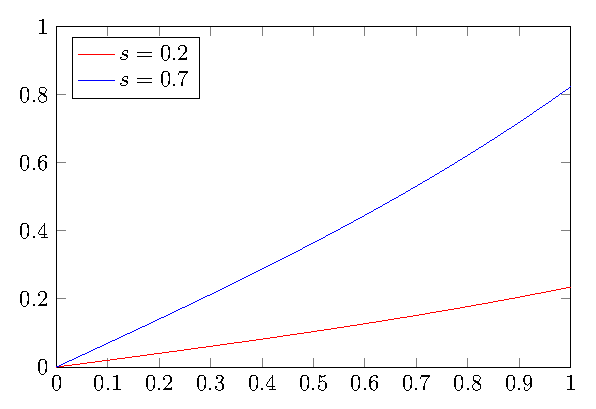
\includegraphics[]{illustrations/plot_s.pdf}
  \caption{Plott av ligning \eqref{eq:ex1a} med forskjellige $s$-verider.}
  \label{fig:s_verdier}
\end{figure}

\noindent Vi ønsker \emph{egentlig} å løse \eqref{eq:ex1eq} med følgende \textbf{rand}betingelser:
\begin{equation}
  y(0) = 0, \; y(1) = 1 \tag{rb}
\end{equation}

I dette tilfellet kan vi, fordi vi kjenner den analytiske løsningen \eqref{eq:ex1a}, se at dette problemet kan løses ved å velge $s=s^*$ slik at $y(1)=s^* \sinh(1)$. Men ettersom vi vanligvis ikke kjenner den analytiske løsningen må vi bruke en annen fremgangsmåte for å finne $s^*$.

For å løse vår ligning må vi velge verdier av $s$ helt til betingelsen $y(1)=1$ er oppfylt. For vilkårlige verdier av $s$ blir $y(1)$ da en funksjon av $s$. Vi starter med å skrive \eqref{eq:ex1eq} som et system:
\begin{align}
  y'(x) &= g(x) \label{eq:ex1sys1} \\
  g'(x) &= y(x) \label{eq:ex1sys2}
\end{align}
Bruker ligning \eqref{eq:phi} og setter
\begin{equation}
  \phi (s) = y(b;s) - \beta = y(1;s) - 1
\end{equation}
der som tidligere nevnt $s=y'(0)=g(0)$. Vi vil nå finne den rette verdien $s=s^*$; det har vi når $\phi(s)=0$.

Vi gjetter nå at $s^{(0)}=0.2, s^{(1)}=0.7$. Dette setter vi inn i ligning \eqref{eq:phi} og får at
\begin{align}
  \phi^{(0)} &= \phi(s^{(0)}) = y(1;s^{(0)}) - 1 \label{eq:exphi1} \\
  \phi^{(1)} &= \phi(s^{(1)}) = y(1;s^{(1)}) - 1 \label{eq:exphi2}
\end{align}
Nå trenger vi en verdi for $y(1;s)$. Det kan vi få ved å bruke f.eks. Eulers metode eller RK4 til å beregne forskjellige verdier for ligngningssystemet \eqref{eq:ex1sys1}, \eqref{eq:ex1sys2}. Ti iterasjoner av Eulers metode med $\Delta x=0.1$ er vist i Tabell \ref{tab:ex1beregn}.

\begin{table}[H]
  \centering
  \caption{}
  \label{tab:ex1beregn}
  \begin{tabularx}{1.0\textwidth}{X|XXXXXXXXX}
    \toprule
    $n$ & 0   & 1    & 2      & 3      &          & 7      & 8     & 9     & 10    \\
    $x$ & 0   & 0.1  & 0.2    & 0.3    & $\cdots$ & 0.7    & 0.8   & 0.9   & 1.0   \\
    \midrule
    y   & 0.0 & 0.1s & 0.20s  & 0.301s &          & 0.735s & 0.856s & 0.985s & 1.122s \\
    y'  & s   & s    & 1.01s  & 1.030s & $\cdots$ & 1.214s & 1.288s & 1.374s & 1.473s \\
    y'' & 0.0 & 0.1s & 0.20s  & 0.301s &          & 0.735s & 0.856s & 0.985s & 1.122s \\
    \bottomrule
  \end{tabularx}
\end{table}

\noindent Setter nå verdien for $y(1)$ fra tabellen inn i ligninene \eqref{eq:exphi1} og \eqref{eq:exphi2}:
\begin{align}
  \phi^{(0)} &= 1.122s^{(0)} - 1 = 1.122 \cdot 0.2 - 1 = -0.7756 \\
  \phi^{(1)} &= 1.122s^{(1)} - 1 = 1.122 \cdot 0.7 - 1 = -0.2146
\end{align}
Dette setter vi nå inn i \eqref{eq:scorr} for å finne en interpolert korrekt verdi for $s$:
\begin{equation}
  s^* = \dfrac{\phi^{(1)}\cdot s^{(0)} - \phi^{(0)}\cdot s^{(1)}}{\phi^{(1)} - \phi^{(0)}}
      = \frac{-0.2146 \cdot 0.2 + 0.7756 \cdot 0.7}{-0.2146+0.7756} = 0.891
\end{equation}
For å sjekke løsningen setter vi den beregnede verdien $s^*$ inn i den analytiske løsningen i ligning \eqref{eq:ex1a} og sjekker om randbetingelsen $y(1) = 1$ holder:
\begin{equation}
  y(1;s^*) = s^* \cdot \sinh(1) = 0.891 \cdot sinh(1) = 1.0471
\end{equation}
Dette er altså en rimelig god tilnærming. Nøyaktigheten kunne vært forbedret ved å bruke RK4 i stedet for Eulers metode.

% section line_re_ligninger (end)


\clearpage
\begin{thebibliography}{1}
  \bibitem{komp} Numeriske beregninger kompendium, \emph{Jan B. Aarseth}
  \bibitem{wolf} Wolfram.com artikkel om løsing av randverdiproblemer: \\ \url{http://reference.wolfram.com/mathematica/tutorial/NDSolveBVP.html}
\end{thebibliography}


\end{document}
